\documentclass{article}
\usepackage{seqsplit}
\usepackage{gensymb}
\usepackage{hyperref}
\usepackage{graphicx}
\def\Version#1{\def\version{#1}}

\date{\today}
\Version{0.4}

\begin{document}
% start of titlepage -- {{{
\begin{titlepage}
	\centering
	{\scshape\Huge Waterloo Rocketry Team \par}
	\vspace{1.5cm}
	{\scshape\bfseries\LARGE Electrical Design and Assembly Standards\par}
	\vspace{2cm}
	{\Large\itshape Aaron Morrison\par}
	{\Large\itshape Alex Mihaila\par}
	\vfill

% Bottom of the page
	{\large \makeatletter\@date\par Revision \version}
    \par
\end{titlepage}
% end titlepage -- }}}

%start of guiding principles section -- {{{
\section{Guiding Principles of all Decisions}
This document exists to set out a standard for all the electrical gear (avionics, telemetry, ground support equipment). Changes/revisions are very welcome. All design decisions on mission critical electrical systems should be made with the following four points in mind:

\begin{enumerate}
\item Our electrical stuff needs to work 100\% of the time at competition. If that's unattainable, 6 sigma is also acceptable. A lot of work from a lot of people go into building this rocket, and missing our 1 launch attempt because of an electrical problem is not acceptable.
\item Once we leave the bay, all electrical work should be done. Fixing something in the desert requires running a generator in a trailer in 40 degree heat. No one does their best work in 40 degree heat. Any MacGyvered solution you come up with there will be orders of magnitude worse than a proper solution you create in Waterloo, and if you're in the desert, there are better things you should be spending your time on.
\item The rest of the team should never be waiting on a fix from us. Electrical stuff should work, and it should work as soon as we need it to. With electrical systems we have the luxury to make sure they work in advance (the engine team does not have this), and we should know all the failure modes and be prepared for them. 
\item We should never be asking another university's team for gear in the desert. Whether or not we fly should not be at the whim of whether we can find something we could have packed a spare of. If something can break, you should have a spare. If there's a tool you need, you should have it with you. We bring everything we need; we shouldn't be asking around for gear.
\end{enumerate}
This document is written in descending order of importance. If you need to decide between whether to follow a guiding principle or a hard rule, follow the principle. As long as your decisions demonstrably don't violate any of these 4, you're probably ok.
%end of guiding principles section -- }}}

%start of hard rules section -- {{{
\section{Rules}
Here are the rules for all the design and assembly decisions. If you want to break one of these rules, make sure you have a very good excuse. Again though, this document was written by someone who doesn't actually have any idea of what he's doing, so if you think a rule is stupid, feel free to cross it out (provide a reason though). If you think a rule is unclear, feel free to elaborate on it. If you think there's a good rule that should be added, please write it in in the margin or pull request the repository (\url{https://github.com/waterloo-rocketry/waterloo\_rocketry\_electrical\_standard}).

%start of connections subsection -- {{{
\subsection{Connections}
\begin{itemize}
\item Don't solder stranded wire to protoboard. Don't solder stranded wire to a connector. It gets brittle and it breaks. Use crimped connections, screw terminals, etc instead.
\item If you're making a crimped connection, use a proper crimp tool if at all possible. Pliers work in a pinch, but the connection is messier and more likely to fail. Good crimp tools are expensive but worth it. (If you're in MME, you can borrow one from MESS.)
\item If you absolutely need to solder stranded core to something, make sure it's very strain relieved (I personally like P clamps, but zip ties work too).
\item Crimped connections should be done on stranded wire only. Don't crimp onto solid core. It's weak and it will break, often when you least want it to.
\item All exposed wire should be heatshrunk; all heatshrink should be clear (IREC regulation).
\item If you screw up a soldering job (we all do it), redo the job. When soldering surface mount components, inspect solder joints with a small magnifying glass.
\item All connections must be tug proof.
\item If a connector could be asymmetric, it should be asymmetric, since asymmetric connectors are much harder to plug in backwards.
\end{itemize}
%end of connections subsection -- }}}

%start of wiring and assembly subsection -- {{{
\subsection{General Wiring \& Assembly}
\begin{itemize}
\item Wiring should be done so that the circuit is as readable as possible. If supplies allow, use different a different insulation color for each wire (at the very least, positive should be red, ground should be black, and all other wires should not be red or black).
\item All wires you use need to be low enough gauge to match the current you're putting through them.
\item If your wires get handled or moved or torqued at any point, they should be strain relieved on both sides of the torque point.
\item Strain relieve everything to the point that it can survive violent shaking (if it's actually going in the rocket, it should survive very violent shaking).
\item Tight wires between two points are accidents waiting to happen. Avoid these.
\item If you're using an RC lithium polymer battery, it should be fused (those fuckers can sink 50 amps).
\item When designing a box, circuit layout, or other assembly, keep in mind that wires and electrical components do take up space. Leave clearance in the design stage; this problem should be solved before fabrication/assembly.
\item Keep good isolation. That means standoffs and that means decent creepage distances.
\item When using shielded cable, ensure the shield is properly terminated and grounded. Shields should only be grounded at one end of the cable.
\end{itemize}
%end of wiring and assembly subsection -- }}}

%start of software subsection -- {{{
\subsection{Software}
\begin{itemize}
\item If your system has any software anywhere, that software should be unit tested.
\item If your system requires a computer program to be used, that program counts as mission critical. It should run on at least two machines and at least two people should be trained to use it.
\item All mission critical software should be expressible (and accompanied by) less than 100 lines of pseudocode.
\item All software should use a VCS (probably git), and all final versions of your software should go with your development logs (see Documentation Standards) on the drive.
\end{itemize}
%end of software subsection -- }}}

%start of pcb subsection -- {{{
\subsection{PCB Design}
\begin{itemize}
\item If your PCBs are meant to be screwed onto something, put mounting holes on your layout, and if at all possible, use M3 screws (for standardization purposes. If you have a space restriction, smaller screws are fine).
\item If a pin is listed as NC on a data sheet, don't pull it to ground. Just leave it unconnected. Some manufacturers (from what stack overflow tells me), use NC pins for in production testing, and as such they aren't actually high impedance pins, and shorting them elsewhere may destroy your IC.
\item Use plated holes for any through-hole components. This is default in most PCB design sofware. If a trace on the bottom and a trace on the top of the board meet at a component lead, the hole, not the lead, should be the conductor between them. Not using plated holes can cause continuity issues if the solder doesn't wick completely through the hole during assembly.
\item If it is reasonable, route traces so that if a solder joint on one component fails (eg. if a pad rips off), it does not affect downstream components (see Figure \ref{powertraces} below). This applies especially to power connections for independent parts of the circuit. Don't daisy chain power lines through the leads or pads of components.

\begin{figure}[h]
    \centering
    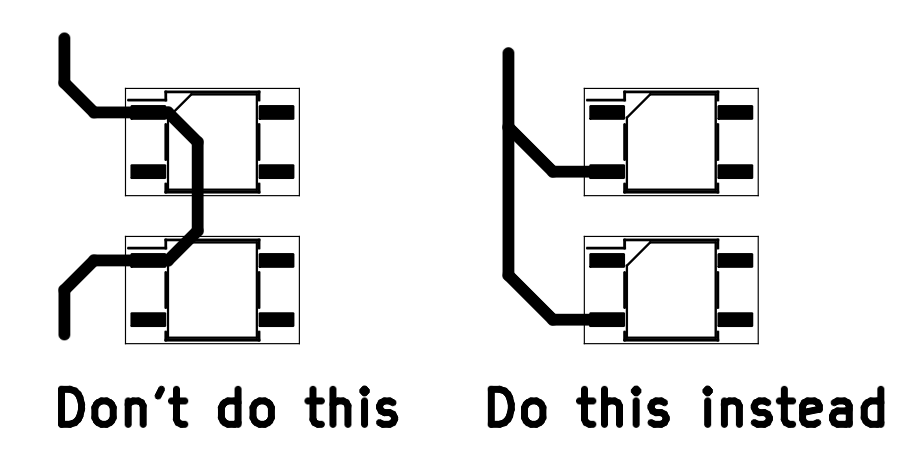
\includegraphics[height=3cm]{power_traces.png}
    \caption{Power trace routing}
    \label{powertraces}
\end{figure}

\item Don't print PCBs at the 3D Printing Center in E5. These are typically poor quality.

\item Points that only apply to designs intended to be handsoldered:
\begin{itemize}
\item Use SMD pads that are longer than you need. KiCad has specific footprints whose names end in \_HandSoldering, which have extended pads for easier hand-soldering (eg don't use footprint "R\_0805", use "R\_0805\_HandSoldering").
\item SOT-23 and 0805 SMT components are quite easily hand-solderable. SOT-23-5 are also doable, but are harder.
\item BGA components can't be hand-soldered. There might exist a reflow oven somewhere on campus that we have access to, but laying paste will be a pain. Avoid BGA packages if you plan to assemble by hand.
\item Don't batch assemble boards (if you are making multiple) when they arrive, because you will be less inclined to change your design if you notice small bugs if you've already committed lots of components (which are worth far more than the cheap boards) to this design. Build one, test to death, then decide whether to make another revision or to assemble the rest.
\end{itemize}
\end{itemize}
%end of pcb subsection -- }}}

%start of miscellaneous subsection -- {{{
\subsection{Miscellaneous}
\begin{itemize}
\item All switches need idiot-proof labeling. Labeling should be permanent (i.e. not tape, etc).
\item All mission critical components should have a hotswappable replacement. You should have that replacement's location written down. "Hotswappable" means you can replace it without any tools (except maybe pliers or a screwdriver. But no generator).
\item If it's conceivably possible for a component to be installed backwards, there should be idiot proof documentation of which way it goes, that documentation should be less than 2 inches from the install point.
\item Buy spares. You will fuck things up, be prepared.
\item Don't solder at hotter than 700\degree. Even that is probably pretty aggressive. Use leaded solder, it melts at a low temperature so you won't burn off all your flux. If your solder isn't melting below 700\degree, the iron's tip is probably bad and should be replaced. Take care of your tips!
\item Don't short things. If you have any bare wires flailing around, don't apply power to the system.
\item All battery connections should be terminated in a female connector to prevent battery shorting and enable easy battery swapping.
\item Before ordering any components, make a list of all components in your design, and go through their data sheets one by one and ensure that they meet or exceed the requirements of your design. Do not just trust the Digikey table values, they are occasionally mislabeled.
\end{itemize}
%end of mescellaneous subsection -- }}}
%end of hard rules section -- }}}

%start of documentation section -- {{{
\section{Documentation Standards}
It is your responsibility to ensure that your project is fully documented and available to the team. Development and documentation for all electrical projects should be tracked in git and hosted on GitHub (under the team organization, waterloo-rocketry). If you manage your repository using issues and pull requests, and if decisions regarding these are made in Slack conversations, put a permalink to the conversation in the issue comment (this is to help traceability). In general, how you manage your project repository is up to you.

Release documentation for each project should also be put in Electrical/$\langle$project folder$\rangle$ on the Drive. Project documentation should include the following:

\begin{enumerate}
\item Users guide
\begin{itemize}
\item Step by step operating instructions.
\item Partway through a procedure, if something can go wrong, say what it is, how you can tell it's gone wrong, and a reference to your troubleshooting guide on how to fix it.
\item Assume that you will not be there when your system is used. Your documentation should be so good that someone who has never seen your system can fix/use it.
\item This probably just needs to be a single checklist/procedure.
\end{itemize}
\item Troubleshooting Guide
\begin{itemize}
\item Include the symptoms of every failure mode, what the worst case scenario is, how to diagnose this failure mode conclusively, and how to fix it.
\item This should have a list of every component in your system, and how to test that component in isolation. This list will be useful for building spares kits.
\end{itemize}
\item Design Documentation
\begin{itemize}
\item A document outlining the major decisions made for your project. The point of this is so that future generations maintaining your project know the reasoning behind your decisions. This can include meeting minutes, block diagrams, or anything else you think would be helpful. If it makes sense to reference slack conversations here, use a permalink to the relevant message.
\end{itemize}
\item Datasheets
\begin{itemize}
\item Self-explanatory. Include datasheets for every component you use.
\end{itemize}
\item Schematics \& Board Layout
\begin{itemize}
\item Any circuit you build should be thoroughly documented in a schematic. Schematics should be correct, clear, and well-organized. The primary purpose of a schematic is to communicate the circuit to someone who hasn't seen it before. A messy schematic will make your circuit harder to review.
\item Some guidelines can be found at \url{https://electronics.stackexchange.com/questions/28251/rules-and-guidelines-for-drawing-good-schematics}.
\item The components in your schematics should match what you intend to use in the circuit. If you are using a particular component, label it as such (and provide a datasheet - see above). This will help identify potential issues in design reviews.
\item If your schematic editor doesn't have a symbol for the part you intend to use, make a custom one (all decent editors support this). Eg. a TL780 voltage regulator should not be represented by a BD244 transistor.
\item Provide both the PDFs and original files for schematics and PCBs.
\end{itemize}
\end{enumerate}
%end of documentation section -- }}}

%start of design guidelines section -- {{{
\section{Design Reviews}
% Expand this into "Design Guidelines" as more stuff accumulates.
If you're designing any part of a system, you should be conducting design reviews. This applies whether there are multiple people working on the system or if you're the only one. If you're alone on a project, this is a good opportunity to make someone else familiar with your work. Apart from resulting in a better circuit, design reviews will also help ensure that you are never the only one who knows how your project should work.
\begin{itemize}
\item  Conduct design reviews on every major revision of your system. This means bringing in another person to discuss your circuit. Keep a record of what was discussed and decided in the review. When presenting a new revision, indicate what has been changed since the last review.
\item Design reviews should be thorough. Even innocent looking sections should be discussed. Chances are you won't find a bug there, but it will save you pain down the line. Discuss failure modes and alternative solutions.
\item The person doing your review should know what they're doing.
\item If appropriate, invite junior members to listen in on the review. They will benefit from being part of the review process and will become better designers and reviewers in the future.
\end{itemize}
%end of design guidelines section -- }}}
\end{document}
